\chapter{Interfaces de usuario: código y GUI}
\label{cap:codigo}

\section{La clase \code{BallPlate}}

\code{BallPlate} tiene la misma interfaz que \code{BallBeam}, con las entradas, referencias y perturbaciones convertidas en vectores de dos componentes. Funciona por lotes (\code{run(T)}) y en vivo (\code{start}/\code{stop}), y ambos modos dan exactamente el mismo resultado.

\begin{figure}[H]
\centering
\resizebox{\linewidth}{!}{%
\begin{tikzpicture}[>=Latex,font=\small,
  ll/.style={draw,thick,minimum width=2.6cm,minimum height=0.8cm,fill=#1,align=center},ll/.default=gray!10,
  lab/.style={above,font=\scriptsize,fill=white,inner sep=1pt}]
\def\xa{0}\def\xb{6.5}\def\xc{13}
\node[ll=c1!12] (u) at (\xa,0) {Usuario /\\script / GUI};
\node[ll=c4!12] (c) at (\xb,0) {\code{BallPlate}};
\node[ll=c5!12] (s) at (\xc,0) {Simulink\\\code{ballplate\_sim}};
\foreach \n in {u,c,s} \draw[dashed,gray] (\n.south) -- ++(0,-8.4);
\draw[->] (\xa,-1.1) -- node[lab]{\code{setMode}, \code{setRef}, \code{setInitialState}} (\xb,-1.1);
\draw[->] (\xb,-1.8) -- node[lab]{\code{set\_param(cmd\_*)}, \code{assignin('base','P')}} (\xc,-1.8);
\draw[->] (\xa,-2.6) -- node[lab]{\code{start()}} (\xb,-2.6);
\draw[->] (\xb,-3.3) -- node[lab]{\code{SimulationCommand=start} (pacing 1x)} (\xc,-3.3);
\draw[->,c2] (\xc,-4.0) -- node[lab]{\code{StartFcn}: \emph{listener} sobre \code{telemetry}} (\xb,-4.0);
\draw[->,c2] (\xc,-4.7) -- node[lab]{\code{PostOutputs} (cada paso)} (\xb,-4.7);
\draw[->,c2] (\xb,-5.4) -- node[lab]{\code{callback(t,d)} hasta 30 Hz} (\xa,-5.4);
\draw[->] (\xa,-6.2) -- node[lab]{\code{push(F,dur)}, \code{setVoltage(Va,Vb)}, \code{setParam(...)}} (\xb,-6.2);
\draw[->] (\xb,-6.9) -- node[lab]{\code{cmd\_dist}, \code{cmd\_ctrl} / \code{SimulationCommand=update}} (\xc,-6.9);
\draw[->] (\xa,-7.7) -- node[lab]{\code{stop(); res = lastResult()}} (\xb,-7.7);
\end{tikzpicture}}
\caption{Secuencia de interacción en el modo en vivo.}
\label{fig:modos}
\end{figure}

\subsection{Referencia de métodos}

\begin{table}[H]
\centering\small
\begin{tabularx}{\linewidth}{@{}p{5.4cm}Xc@{}}
\toprule
Método & Descripción & En vivo\\
\midrule
\code{bp = BallPlate()} & Carga (o genera) el modelo y calcula las ganancias de ambos ejes. & --\\
\code{res = bp.run(T)} & Simulación por lotes de $T$ segundos. & no\\
\code{bp.start()}, \code{stop()}, \code{pause()}, \code{resume()} & Control de la simulación en vivo. & --\\
\code{bp.setMode(m)} & \code{'open'}, \code{'plate'}, \code{'cascade'}, \code{'lqr'} (o 0..3). & sí\\
\code{bp.enable(tf)} & Habilita o inhibe el controlador. & sí\\
\code{bp.setVoltage(Va, Vb)} & Tensiones manuales [V], sumadas a las del controlador. & sí\\
\code{bp.setPlateAngle(al, be)} & Inclinaciones para el modo \code{'plate'} [rad]. & sí\\
\code{bp.setRef(tipo, [cx cy], A, f)} & \code{'point'}, \code{'circle'}, \code{'square'}, \code{'eight'}, \code{'external'} (m, Hz). & sí\\
\code{bp.push([Fx Fy], dur)} & Golpecito sobre la bola [N, s]. & sí\\
\code{bp.setParam(nombre, valor)} & Cambia un parámetro y recalcula magnitudes derivadas y ambos LQR. & sí$^*$\\
\code{bp.setParamRaw(nombre, valor)} & Cambia un parámetro \emph{sin} recalcular nada. & sí$^*$\\
\code{bp.setInitialState(s0)} & Estado de 8 componentes para el próximo arranque. & no\\
\code{bp.setRefSignal(t, rxy)} & Referencia externa, \code{rxy} de $N\times2$. & no\\
\code{bp.setVoltageSignal(t, U)} & Tensiones adicionales programadas, $N\times2$. & no\\
\code{bp.setDisturbanceSignal(t, F)} & Fuerzas programadas sobre la bola, $N\times2$. & no\\
\code{bp.addTelemetryCallback(f)} & Registra \code{f(t,d)}, con \code{d} el vector de la tabla~\ref{tab:tel}. & --\\
\code{res = bp.lastResult()}, \code{bp.animate(res, vel)} & Última sesión en vivo; reproducción en 3D. & --\\
\bottomrule
\end{tabularx}
\caption{API de \code{BallPlate}. ($^*$) Excepto \code{Tcam} y \code{cam\_delay}, que se aplican en el siguiente arranque.}
\end{table}

\subsection{Ejemplos}

\begin{ejemplo}{Movimiento punto a punto: LQR frente a cascada}
\begin{lstlisting}
bp = BallPlate();
t = [0 1 1.001 6]';  rxy = [0 0; 0 0; 0.08 -0.05; 0.08 -0.05];
bp.setInitialState(zeros(8,1)); bp.setRefSignal(t, rxy);
for m = {'lqr', 'cascade'}
    bp.setMode(m{1}); res = bp.run(6);
    plot(res.x_cm, res.y_cm, 'DisplayName', m{1}); hold on
end
axis equal; legend; xlabel('x [cm]'); ylabel('y [cm]')
\end{lstlisting}
\end{ejemplo}

\begin{ejemplo}{Trayectoria propia: una espiral}
\begin{lstlisting}
t = (0:0.01:20)';  rho = 0.02 + 0.004*t;  th = 2*pi*0.2*t;
bp.setRefSignal(t, [rho.*cos(th), rho.*sin(th)]);
bp.setMode('lqr'); bp.setInitialState([0.02 0 0 0 0 0 0 0]);
res = bp.run(20); bp_plot_results(res, 'Espiral'); bp.animate(res);
\end{lstlisting}
\end{ejemplo}

\begin{ejemplo}{Sesión en vivo desde un script}
\begin{lstlisting}
bp.setMode('lqr'); bp.setRef('point', [0 0]);
bp.TelemetryRate = 2;
bp.addTelemetryCallback(@(t,d) fprintf('t=%5.2f (%+5.1f, %+5.1f) cm\n', ...
    t, 100*d(BallPlate.TEL.x), 100*d(BallPlate.TEL.y)));
bp.start();                              pause(3)
bp.setRef('circle', [0 0], 0.06, 0.2);   pause(6)
bp.push([0 0.3], 0.05);                  pause(3)
bp.stop(); res = bp.lastResult(); bp.clearCallbacks();
\end{lstlisting}
\end{ejemplo}

\section{Interfaz gráfica \code{bp\_gui}}

\code{bp\_gui} abre una ventana con dos vistas del sistema (figura~\ref{fig:gui}): a la izquierda la escena 3D y a la derecha la \textbf{vista de la cámara}, una vista cenital del plato con la bola, su estela y la referencia. \textbf{Un clic en la vista de la cámara lleva la referencia a ese punto}: es la forma más rápida de jugar con el sistema. Debajo, las gráficas en vivo de $x$, $y$ y sus referencias, de las inclinaciones y de las tensiones.

\begin{figure}[H]
\centering
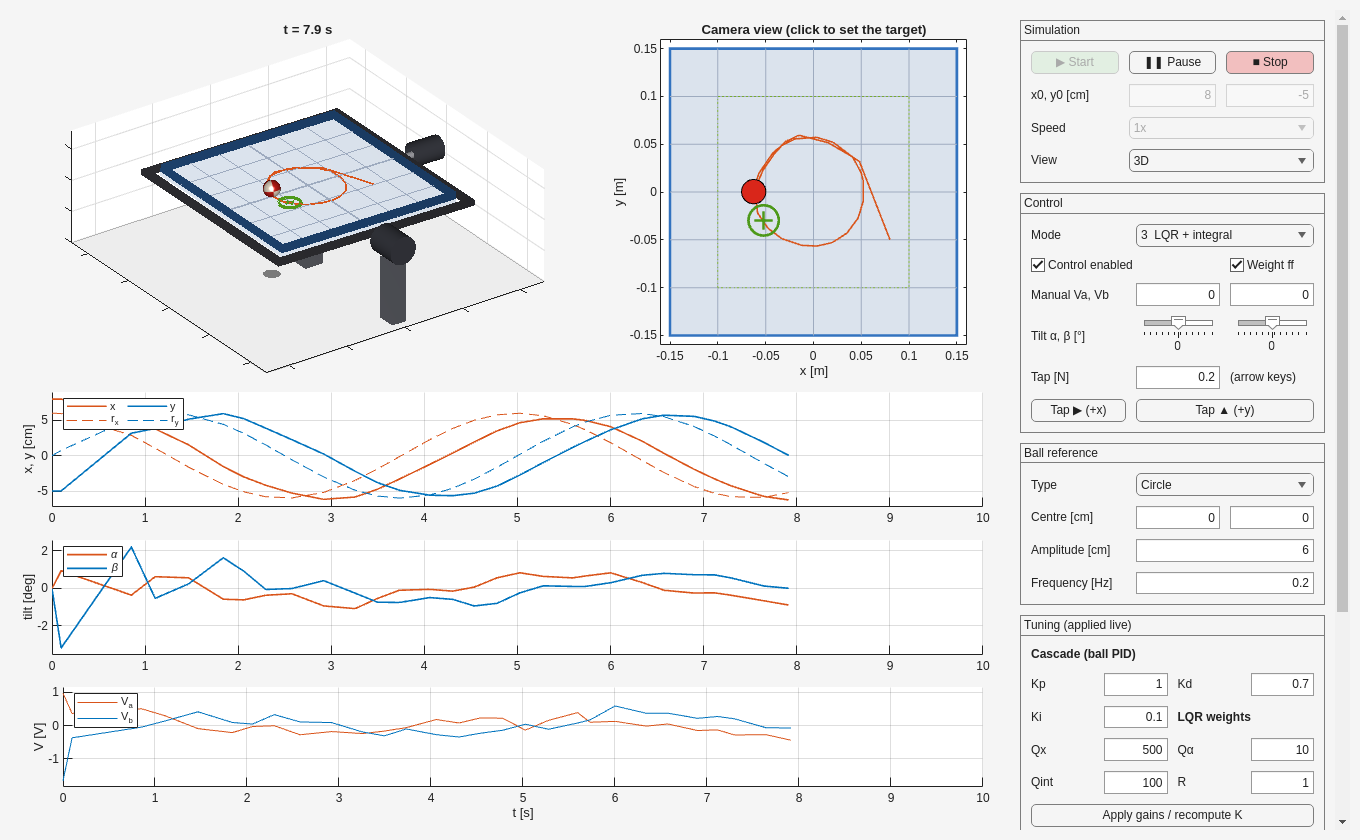
\includegraphics[width=\linewidth]{data/gui.png}
\caption{La GUI siguiendo en vivo una circunferencia con el LQR.}
\label{fig:gui}
\end{figure}

\paragraph{La escena 3D.} La dibuja \code{bp\_draw}: la base y el poste central, el motor A (fijo), el marco exterior de la cardán, que solo gira con $\alpha$, el motor B montado sobre él y el plato con una rejilla de \SI{5}{cm}, que gira con $\alpha$ y $\beta$. La bola tiene dos colores para que se vea rodar y deja una estela corta y una sombra sobre la base; el anillo verde es la referencia. Las vistas predefinidas (\code{bp\_view}) son 3D, \emph{Top}, \emph{Front} (muestra $\alpha$ en verdadera magnitud) y \emph{Side} (muestra $\beta$).

\paragraph{Uso típico.}
\begin{enumerate}
  \item Elegir la posición inicial de la bola, la velocidad de simulación y los fotogramas por segundo de la cámara (se aplican al pulsar \textbf{Start}).
  \item Pulsar \textbf{Start}. Modo, referencia, tensiones, ganancias y pesos se cambian en vivo.
  \item Hacer clic en la vista de la cámara para mover el objetivo, o elegir una trayectoria (circunferencia, cuadrado, ocho) con su centro, amplitud y frecuencia.
  \item Con la ventana activa, las flechas del teclado dan un golpecito a la bola en esa dirección.
  \item \textbf{Stop} y \textbf{Export last run}: los datos quedan en \code{bp\_res} y se representan con \code{bp\_plot\_results}.
\end{enumerate}
